% The 2-cell of the torus, attached via the word a b a^{-1} b^{-1}.
% Source: book/tex/topology/constructions.tex (§ The torus).
\documentclass[border=2mm]{standalone}
\usepackage{tikz}
\usetikzlibrary{arrows.meta,decorations.markings}
\tikzset{midarr/.style={decoration={markings,
  mark=at position 0.5 with {\arrow{Latex[length=2mm]}}},postaction={decorate}}}
\begin{document}
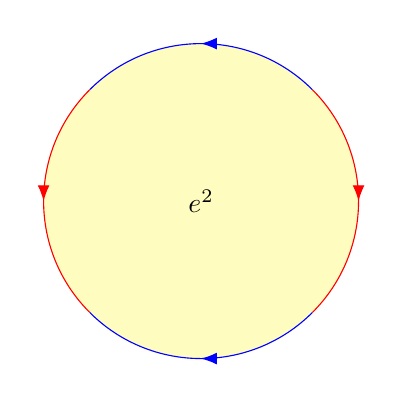
\begin{tikzpicture}[scale=2]
  \fill[yellow!25] (0,0) circle (1);
  \draw[blue, midarr] (45:1) arc (45:135:1);   % top
  \draw[blue, midarr] (315:1) arc (315:225:1); % bottom
  \draw[red, midarr] (135:1) arc (135:225:1);  % left
  \draw[red, midarr] (45:1) arc (45:-45:1);    % right
  \node at (0,0) {$e^2$};
\end{tikzpicture}
\end{document}
